%Incidencia de una onda plana a 45° con n_i = 1, n_t = 1.46   

\documentclass[tikz,crop]{standalone}

\usepackage{tikz}
\usetikzlibrary{decorations.pathreplacing,decorations.pathmorphing}
\usepackage{physics}

\begin{document}


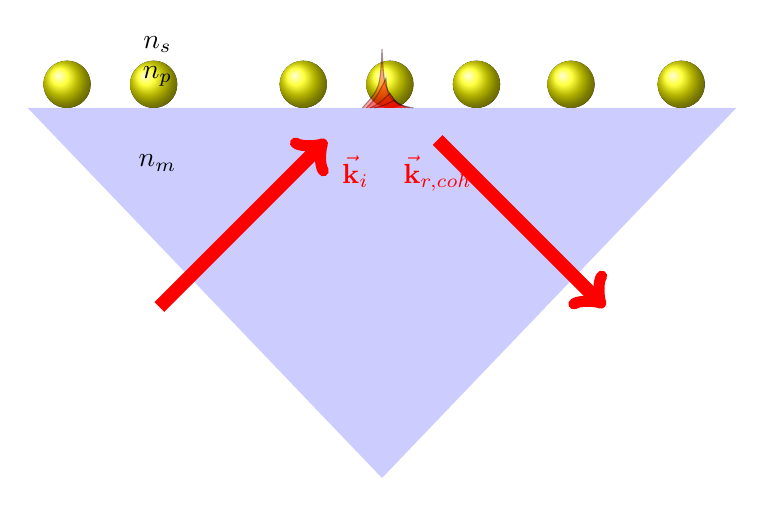
\begin{tikzpicture}%[   ESTO PONE LAS RAYAS QUE USO EN EPSEJOS
%    interface/.style={
        % The border decoration is a path replacing decorator. 
        % For the interface style we want to draw the original path.
        % The postaction option is therefore used to ensure that the
        % border decoration is drawn *after* the original path.
%        postaction={draw,decorate,decoration={border,angle=-45,
%                    amplitude=0.3cm,segment length=2mm}}},
%    ]



%-------------------------------------------- Incidence media


\def\a{.3}
\def\d{.3}

\fill[blue, opacity = .2] (0,-5)--(4.5,-\d)--(-4.5,-\d);


\foreach \x in {-4,-2.9,-1,.1,1.2,2.4,3.8}{
\fill[ball color=yellow, opacity=1] (\x,0) circle(\a);}


%\draw[thick, dashed] (-4.5,0)--(4.5,0);
%\draw[thick, dashed] (-4.5,-\d) rectangle (4.5,\d);

\draw[->, thick, red, line width=5](225:4)--(225:1) node[anchor= north west]{$\va{k}_i$};
\draw[<-, thick, red, line width=5](-45:4)--(-45:1)node[anchor=north ]{$\va{k}_{r,coh}$};



\draw[fill = red, opacity = .35] (-.25,-\d) ..controls (-.025,.25-\d) .. (0,.75-\d)
											..controls (.025,.25-\d) .. (.25,-\d);  %1st evanescent wave
\draw[fill = red, opacity = .35] (-.2,0-\d) ..controls (-.075,.125-\d) .. (0.05,.375-\d)
											..controls (.075,.125-\d) .. (.3,0-\d);  %2nd evanescent wave
\draw[fill = red, opacity = .35] (-.15,0-\d) ..controls (-.025,.0625-\d) .. (0.1,.1875-\d)
											..controls (.175,.0625-\d) .. (.35,0-\d);  %3rd evanescent wave
\draw[fill = red, opacity = .35] (-.1,0-\d) ..controls (.025,.03125-\d) .. (0.15,.09375-\d)
											..controls (.225,.03125-\d) .. (.4,0-\d);  %4th evanescent wave	



\node at (-2.9,.5) {$\; n_s$};
\node at (-2.9,.1) {$\; n_p$};
\node at (-2.9,-1) {$\; n_m$};

\end{tikzpicture}


\end{document}